\documentclass[aspectratio=169,compress,14pt]{beamer}
\usepackage{graphicx}
\graphicspath{ {./images/} }
\usepackage{microtype}
\usepackage[english]{babel}

\DeclareMathAlphabet{\mathfrak}{U}{euf}{m}{n}
\DeclareMathAlphabet{\mathcal}{OMS}{cmsy}{m}{n}
\usepackage[lining,scaled=.9]{FiraMono}
\usepackage[scaled=.98,sups]{XCharter}
\usepackage[charter,vvarbb,scaled=1.05]{newtxmath}
\usepackage{fontawesome}
\usefonttheme{professionalfonts}

\usepackage{booktabs}
% For column-wise revealing of tabular
\usepackage{array}

% \widthof
\usepackage{calc}

\useinnertheme{rectangles}
\setbeamertemplate{sections/subsections in toc}[square]
\defbeamertemplate{itemize item}{squarep}{\hbox{\raisebox{.15ex}{\vrule width 1ex height 1ex}}}
\defbeamertemplate{itemize subitem}{squarep}{\small\hbox{\vrule width 1ex height 1ex}}
\defbeamertemplate{itemize subsubitem}{squarep}{\small\hbox{\vrule width 1ex height 1ex}}
\setbeamertemplate{items}[squarep]

\defbeamertemplate*{title page}{titlepage}[1][]{
  \vbox{}
  \vfill
  \begingroup
  \begin{beamercolorbox}[wd=\paperwidth,sep=8pt,center,#1]{title}
    \parbox{.95\textwidth}{%
      \begin{flushright}
        \bigskip
        {\usebeamerfont{title}\inserttitle\par}
        {\usebeamerfont{author}\insertauthor}
      \end{flushright}%
    }%
    \begin{center}
      \makebox[0pt]{
\includegraphics[width=.95\paperwidth]{lecture.png}}
    \end{center}
  \end{beamercolorbox}%
  \endgroup
  \vfill
  {\centering\tiny These next few slides were defiantly typeset in \LaTeX{} to appease one peculiar zealot's software preferences.\par}
}

\definecolor{dark}{HTML}{181818}
\definecolor{light}{HTML}{e0e0e0}
\definecolor{accent}{HTML}{802626}
\definecolor{fgaccent}{HTML}{993131}

\setbeamercolor{background canvas}{bg=light}
\setbeamercolor{title}{fg=light,bg=dark!90!light}
\setbeamerfont{title}{series=\large\bfseries}
\setbeamerfont{author}{series=\small}
\setbeamercolor{structure}{fg=dark}
\setbeamercolor{alerted text}{fg=fgaccent}
\setbeamercolor{block title}{fg=light,bg=dark!90!light}
\setbeamercolor{block body}{bg=light!90!dark}

\setbeamertemplate{navigation symbols}{}

\newcommand{\TODO}[1]{\colorbox{red}{\textcolor{white}{TODO}}: #1}

\newcommand{\itemvdots}{\item[{\makebox[\widthof{\usebeamertemplate{itemize item}}]{\vdots}}] \mbox{}}

\title{Predicting train delays based on weather data}
\author{\mbox{Arkadiusz Kozdra}, \mbox{Krystyna Korzonek}, \mbox{Patrycja Balik}}

\begin{document}
\begin{frame}[plain]
  \titlepage
\end{frame}

\begin{frame}{The Data}
  \begingroup
  \setlength{\tabcolsep}{10pt}
  \begin{tabular}{@{\onslide<2->}p{.49\textwidth}<{\onslide<3->}|p{.5\textwidth}@{\onslide}}
    \raisebox{-.5\height}{
\includegraphics[width=\linewidth]{imgw.pdf}}\medskip

    {\footnotesize\url{danepubliczne.imgw.pl}} \bigskip%
    &%
    {\large\bfseries InfoPasażer Archiver}

    {\footnotesize\url{ipa.lovethosetrains.com}\linebreak
    (scraped from \url{infopasazer.intercity.pl})} \bigskip\\
    % \#Weather stations \(=\) 67

    Daily weather data:
    \begin{itemize}
      \item mean temperature,
      \item total precipation,
      \item snow cover height,
      \item hail duration in hours,
      \itemvdots
    \end{itemize}%
    &%
    % \#Railway stations \(\approx\) 2300
    Segments with:
    \begin{itemize}
      \item a pair of stations,
      \item arrival delay,
      \item departure delay.
    \end{itemize}
    \onslide<4->{\dots But missing the coordinates!\medskip}
    \onslide<5->{%
      + \raisebox{-.35\height}{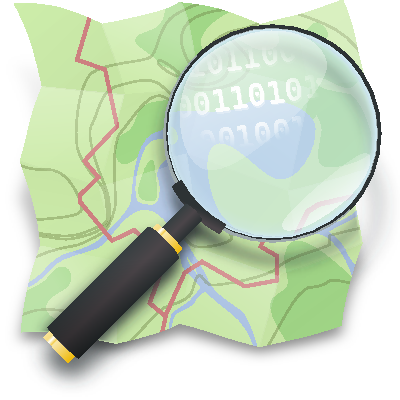
\includegraphics[height=1.5\baselineskip]{osm.pdf}}
      \textbf{OpenStreetMap}}
  \end{tabular}
  \endgroup
\end{frame}

\begin{frame}
  \frametitle<1>{The Data: 67 weather stations}
  \frametitle<2>{The Data: \textasciitilde 2300 railway stations}
  \frametitle<3>{The Data}
  \centering
  \includegraphics<1>[height=.8\textheight]{weather.pdf}%
  \includegraphics<2>[height=.8\textheight]{railway.pdf}%
  \includegraphics<3>[height=.8\textheight]{weather_railway.pdf}
\end{frame}

\begin{frame}{The Data}
  \Large
  \begin{equation*}
    \operatorname{weather}(P) =
    \frac{
      \sum\nolimits_{m \in \textbf{Meteo}} \operatorname{w}_P(m) \cdot m[\operatorname{features}]
    }{
      \sum\nolimits_{m \in \textbf{Meteo}}\operatorname{w}_P(m)
    }
  \end{equation*}
  \bigskip\pause

  \begin{equation*}
    \operatorname{w}_P(m) = e^{-\operatorname{dist}(m[\operatorname{coords}],\, P)}
  \end{equation*}
\end{frame}

\begin{frame}{The Data}
  \huge
  \centering
  \begin{tabular}{c|c}
    \(X\) & \(y\) \\\hline
    \raisebox{-.3cm}{\faSunO \: \faCloud} & \raisebox{-.3cm}{\faTrain \kern1pt \faClockO}
  \end{tabular}
\end{frame}

\begin{frame}{Prediction}
  \TODO{some problems (skewed data and whatever)}
\end{frame}

\begin{frame}{Results}
  \TODO{results, which tools we used and to what effect}
\end{frame}

\begin{frame}{What have we learned?}
  Seeking appropriate data and processing it into a~usable format takes a lot of time.
  \vfill\pause

  Real-life data rarely has a~nice distribution.
  \vfill\pause

  It can be hard to find techniques applicable to regression problems, as
  opposed to classification.
\end{frame}

\begin{frame}{}
  \TODO{colab link thing}
\end{frame}

\end{document}
